% !TeX root = TeX-Talk.tex
% !TeX encoding = UTF-8
% !TeX program = XeLaTeX
\begin{frame}
\begin{tikzpicture}[overlay]
\pgfmathdeclarerandomlist{symbols}{%
  {\texttt{\string\title}}%
  {$\sum A_n$}{$\int d\alpha$}{$\pi$}{$\sqrt2$}{\TeX}{\BibTeX}}
\foreach \y in {0,-1,...,-7} {
  \foreach \x in {0,1,...,12} {
    \pgfmathrandomitem{\randsymbol}{symbols}
    \node[black!15,rotate=45] at (\x,\y) {\randsymbol};
  }
}
\node at (2,-5) {
\includegraphics{tex.pdf}};
\node at (10,-5) {
\includegraphics{meta.pdf}};
\end{tikzpicture}
\titlepage
\end{frame}

\begin{frame}{谈谈历史}{高教授和蓝博士}
\begin{columns}
\column{.5\textwidth}
\begin{figure}
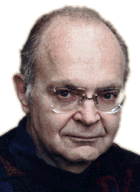
\includegraphics[height=3cm]{don.png}
\caption{\normalparagraph
高德纳(Donald Knuth), Stanford 大学计算机程序设计艺术荣誉教授,Turing 奖得主。为了写他的七卷本著作《The Art of Computer Programming》而编制了 \TeX{} 排版系统。但或许因为在 \TeX{} 上花的十年时间太长,这部著作至今才写到第四卷。}
\end{figure}

\column{.5\textwidth}
\begin{figure}
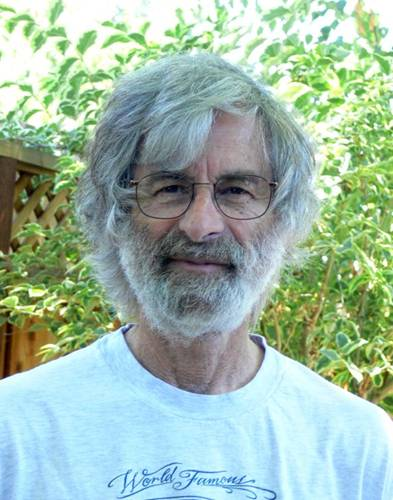
\includegraphics[height=3cm]{leslie.jpg}
\caption{\normalparagraph
Leslie Lamport,微软研究院资深研究员,Turing 奖得主。为了准备他的著作《The Great American Concurrency Book》而编写了一组基于 \TeX{} 的宏,即 \LaTeX{},后交给 \LaTeX3 小组,逐渐发展演变为现在的样子。但是,那部著作一直没有动笔。}
\end{figure}
\end{columns}
\strut
\end{frame}

\begin{frame}{印象里 \TeX/\LaTeX{} 大概是什么?}
\begin{itemize}[<+->]
\item 写毕业论文,据说很方便
\item 论文投稿要用,别的格式不要
\item 写书的工具,有的老师用它
\item 可以写作业、记笔记,输出 PDF
\end{itemize}
\end{frame}

\begin{frame}{人们说 \TeX/\LaTeX{} 是什么?}
\only<3->{\color{gray}}
\TeX{} 来自 technology 的希腊词根 $\tau\epsilon\chi$,读音 \textipa{[tEx]}

$\text{\LaTeX} = \text{Lamport \TeX}$,读音 \textipa{["lA:tEx\*; "leitEx]} 或者随便
\pause
\begin{itemize}
\only<3->{\color{gray}}
\item
\TeX{} 是一种专业排版软件。与它在各方面最为类似的是方正的书版;功能相近而用法不大相同的有方正飞腾创意,Adobe 的 PageMaker、InDesign 等。
\item
\TeX{} 是一种计算机宏语言。同为宏语言的有 C 语言预处理宏、Linux 下的 M4;但功能和形式更相近的是 HTML+PHP。
\item
\LaTeX{} 是定义在 \TeX{} 语言上的一大组宏命令,一种格式。它提供了结构化的方式使得书籍文章可以方便地按内容的逻辑结构进行排版。\LaTeX{} 之于 \TeX{} 类似 HTML+CSS 之于基本的 HTML。
\end{itemize}
\pause

\begin{tikzpicture}[overlay]
\draw[line width=0.5cm, red!50!black] (0,0) -- (12,6) (12,0) -- (0,6);
\end{tikzpicture}
\end{frame}


\begin{frame}[fragile]{\LaTeX{} 到底是什么?——从左到右的转换}
\begin{columns}
\column{.5\textwidth}
\begin{Verbatim}[fontsize=\footnotesize,frame=single]
\documentclass{ctexart}
\usepackage{amsmath}
\usepackage{graphicx}
\title{再论商高之勾股定理}
\author{赵爽}

\begin{document}
\maketitle
句股各自乘,併之為弦實,開方除之即弦。
\cite{zhou}
\begin{gather}\label{eq:gougu}
  c = \sqrt{a^2 + b^2}
\end{gather}
% 其中省略若干行
\bibliographystyle{plain}
\bibliography{chinabib}
\end{document}
\end{Verbatim}
\rule{0pt}{2cm}
\pause
\column{.5\textwidth}
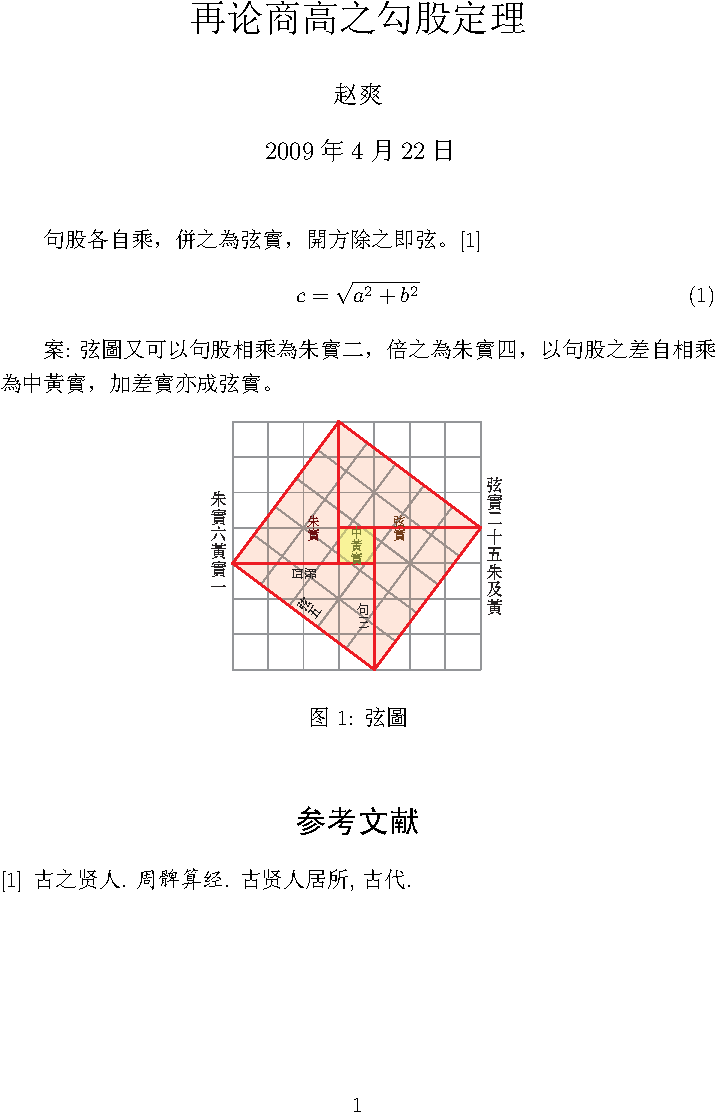
\includegraphics[width=\textwidth]{gougu-crop.pdf}
\end{columns}
\pause
\begin{tikzpicture}[overlay,font={\Huge\bfseries},color=red!50!black]
\node (code) at (2.5,6) {格式化的代码};
\node (paper) at (9.5,6) {排好的文档};
\draw[-latex,line width=0.2cm] (code) -- (paper);
\end{tikzpicture}
\end{frame}

\begin{frame}{安装并更新 \TeX{} 发行版软件}
\begin{itemize}
  \item \TeX Live 2019(每年夏天更新),macOS 下称为 MacTeX 2019
  \item MiKTeX 2.9(Windows)
  \item 网页在线版 \url{https://www.overleaf.com/}
\end{itemize}
各个大学的毕业论文模板可能需要更新 \TeX{} 发行版后才能使用。如果不要求最新,Linux 环境下也可以使用软件源里的版本(APT 大法)。
\end{frame}

\begin{frame}{准备一些靠谱的教程}
\begin{itemize}
\item 英文:印度 TUG 的 \LaTeX{} Tutorials: A Primer——简明实用\\
{\small\url{https://www.tug.org/twg/mactex/tutorials/ltxprimer-1.0.pdf}}
\item 中文:黄新刚的 \LaTeX{} Notes——生动有趣
\url{http://dralpha.altervista.org/zh/tech/lnotes2.pdf}
\item 英文书籍:A Guide to \LaTeX, 4ed(影印版《LaTeX 实用教程》)\\
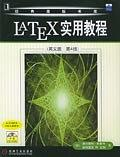
\includegraphics[width=1.5cm]{guide-to-latex.jpg}
\item 中文书籍:本人的《\LaTeX 入门》\\
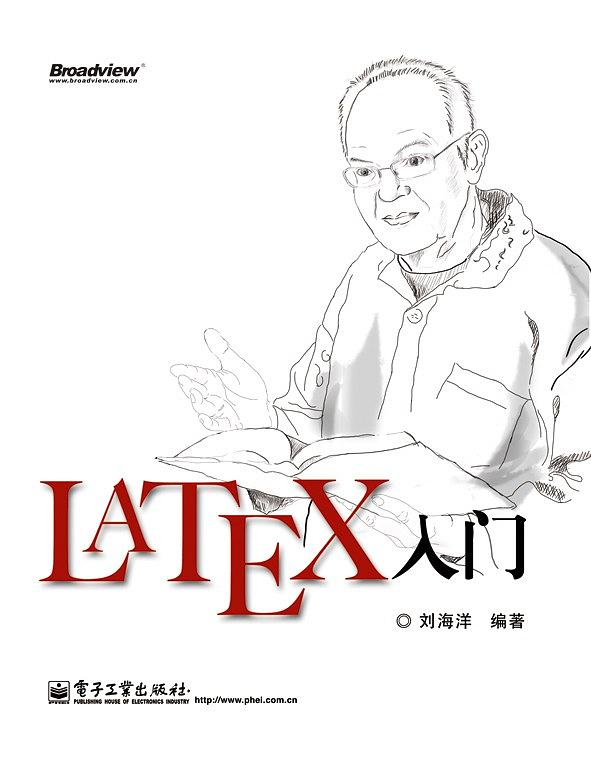
\includegraphics[width=1.5cm]{latexbook.jpg}
\end{itemize}
\end{frame}

\begin{frame}{了解从哪儿解决疑难}
\begin{itemize}
\item 在线手册:在你电脑上用 texdoc 命令调出,或 \url{https://texdoc.net/}
\item 周围熟悉 \LaTeX{} 的人
\item 英文社区:\url{http://tex.stackexchange.com} 等
\item 中文社区:\LaTeX{} 工作室等
\end{itemize}

\end{frame}